\chapter{Phase Retrieval}
The problem of missing phase information is well known and is called the phase problem. There are many ways to overcome it: for example in crystallography homology modelling or the anomalous scattering of heavy atoms is exploited to retrieve phases. Holography uses the interference between two wave fields to obtain the phases. Ptychography uses the precisely known overlap and high redundancy between many exposures to solve the phase problem. CXI makes use of the fact that pnCCD detectors so-called oversample the diffraction pattern, which means that phases can under certain conditions be retrieved from the intensity pattern itself. The next sections will describe oversampling in more detail, explain how phases can be retrieved from an oversampled signal using an iterative phase retrieval method, and finally how phase retrieval can be validated. 

\section{Oversampling} 
In 1952 Sayre noticed that the Bragg peaks sample the molecular transform $\mathcal{F}(H)$ at the critical sampling rate ($S_C$)\cite{Sayre1952a} (See Shannon \cite{Shannon1949a}). This means that knowing the phases belonging to the Bragg peaks is just enough to back-calculate the structure of the measured object. Single particle imaging is free from the crystal lattice, and isolated Bragg peaks give way to a continuous diffraction pattern. By choosing the detector distance appropriately such that individual pixels cover a small enough angle, we can sample the molecular transform more finely than the critical sampling rate. This sampling condition is called oversampling. Figure \ref{fig:sampling} illustrates both cases of sampling. 

\begin{figure}[h]
	\centering 
		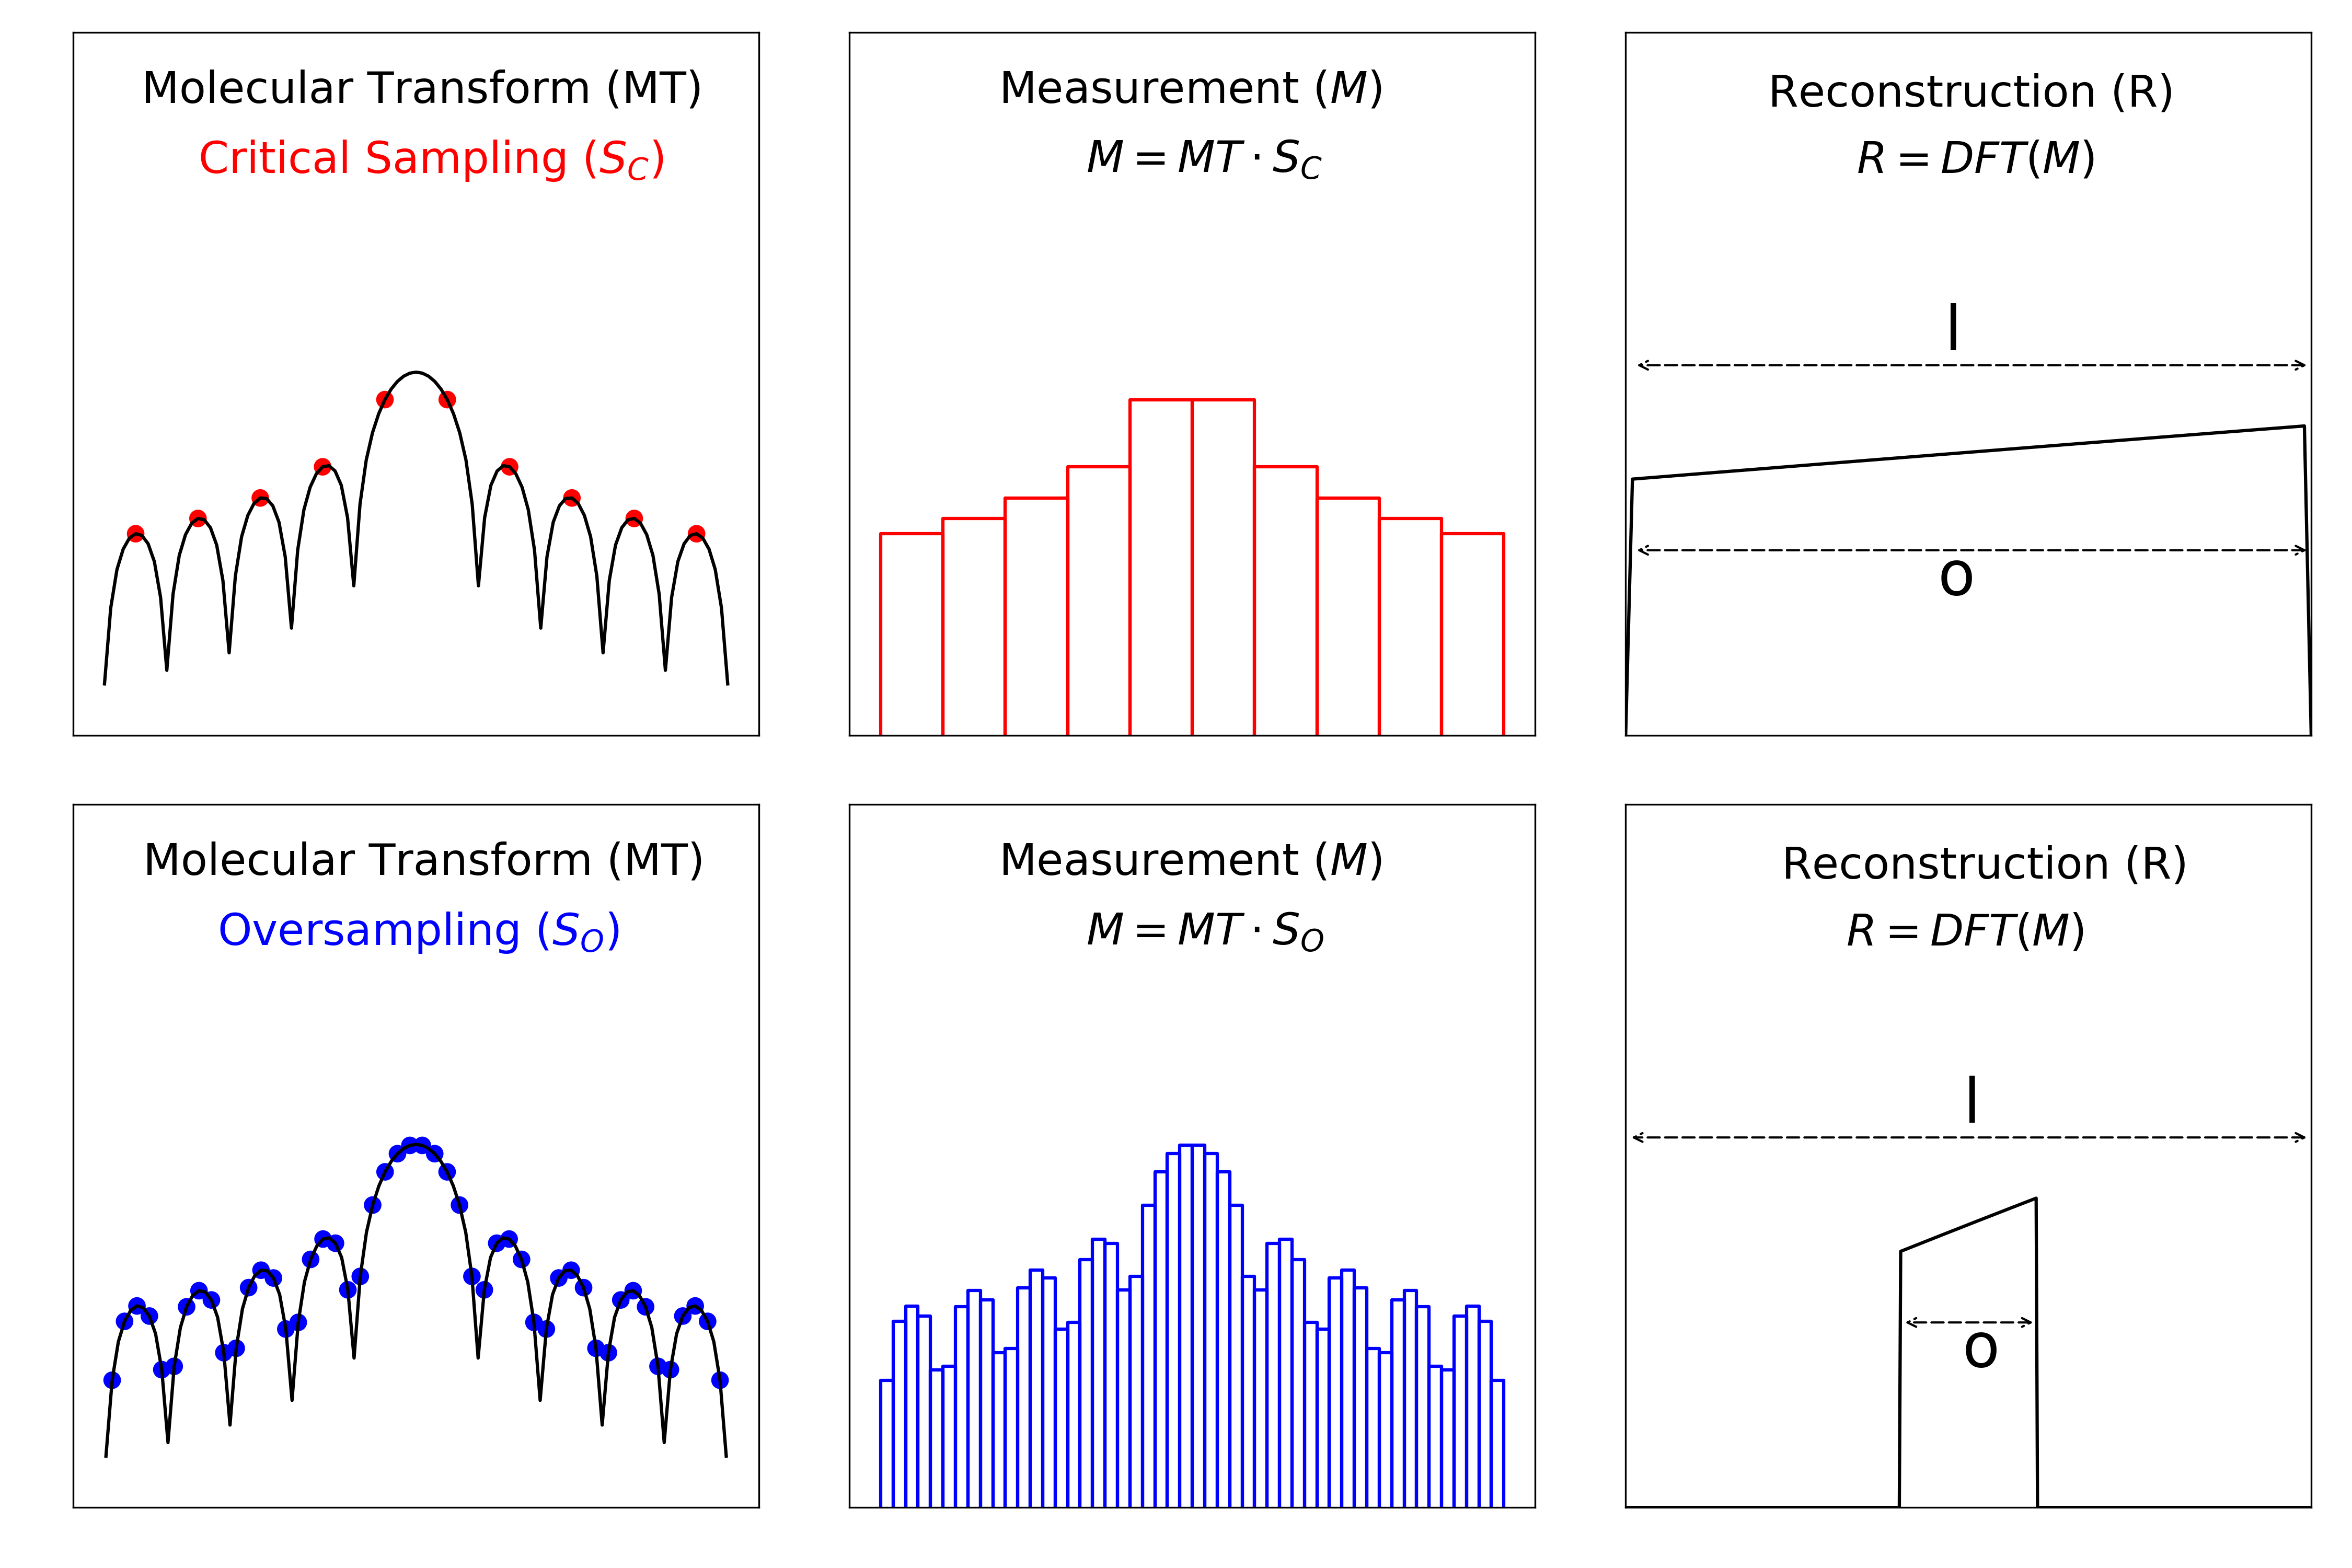
\includegraphics[width=120mm]{sampling.png}
	\caption{Illustration of critical sampling versus 		oversampling.}
	\label{fig:sampling}
\end{figure}

The linear sampling rate $S$ is defined as the ratio of $l/o$, where $l$ is the window size, and $o$ is the object size. Due to the inverse relation between the object and the molecular transform $l = \frac{1}{q} = \frac{\lambda\, d}{p}$, where $q$ is a 'pixel' in F(S) (see equation \ref{eq:q}. 
\begin{equation}
S = \frac{\lambda\,d}{o\,p}
\end{equation}

Figure \ref{fig:sampling} illustrates two types of sampling: critical sampling, and oversampling.

\begin{figure}[h]
	\centering 
		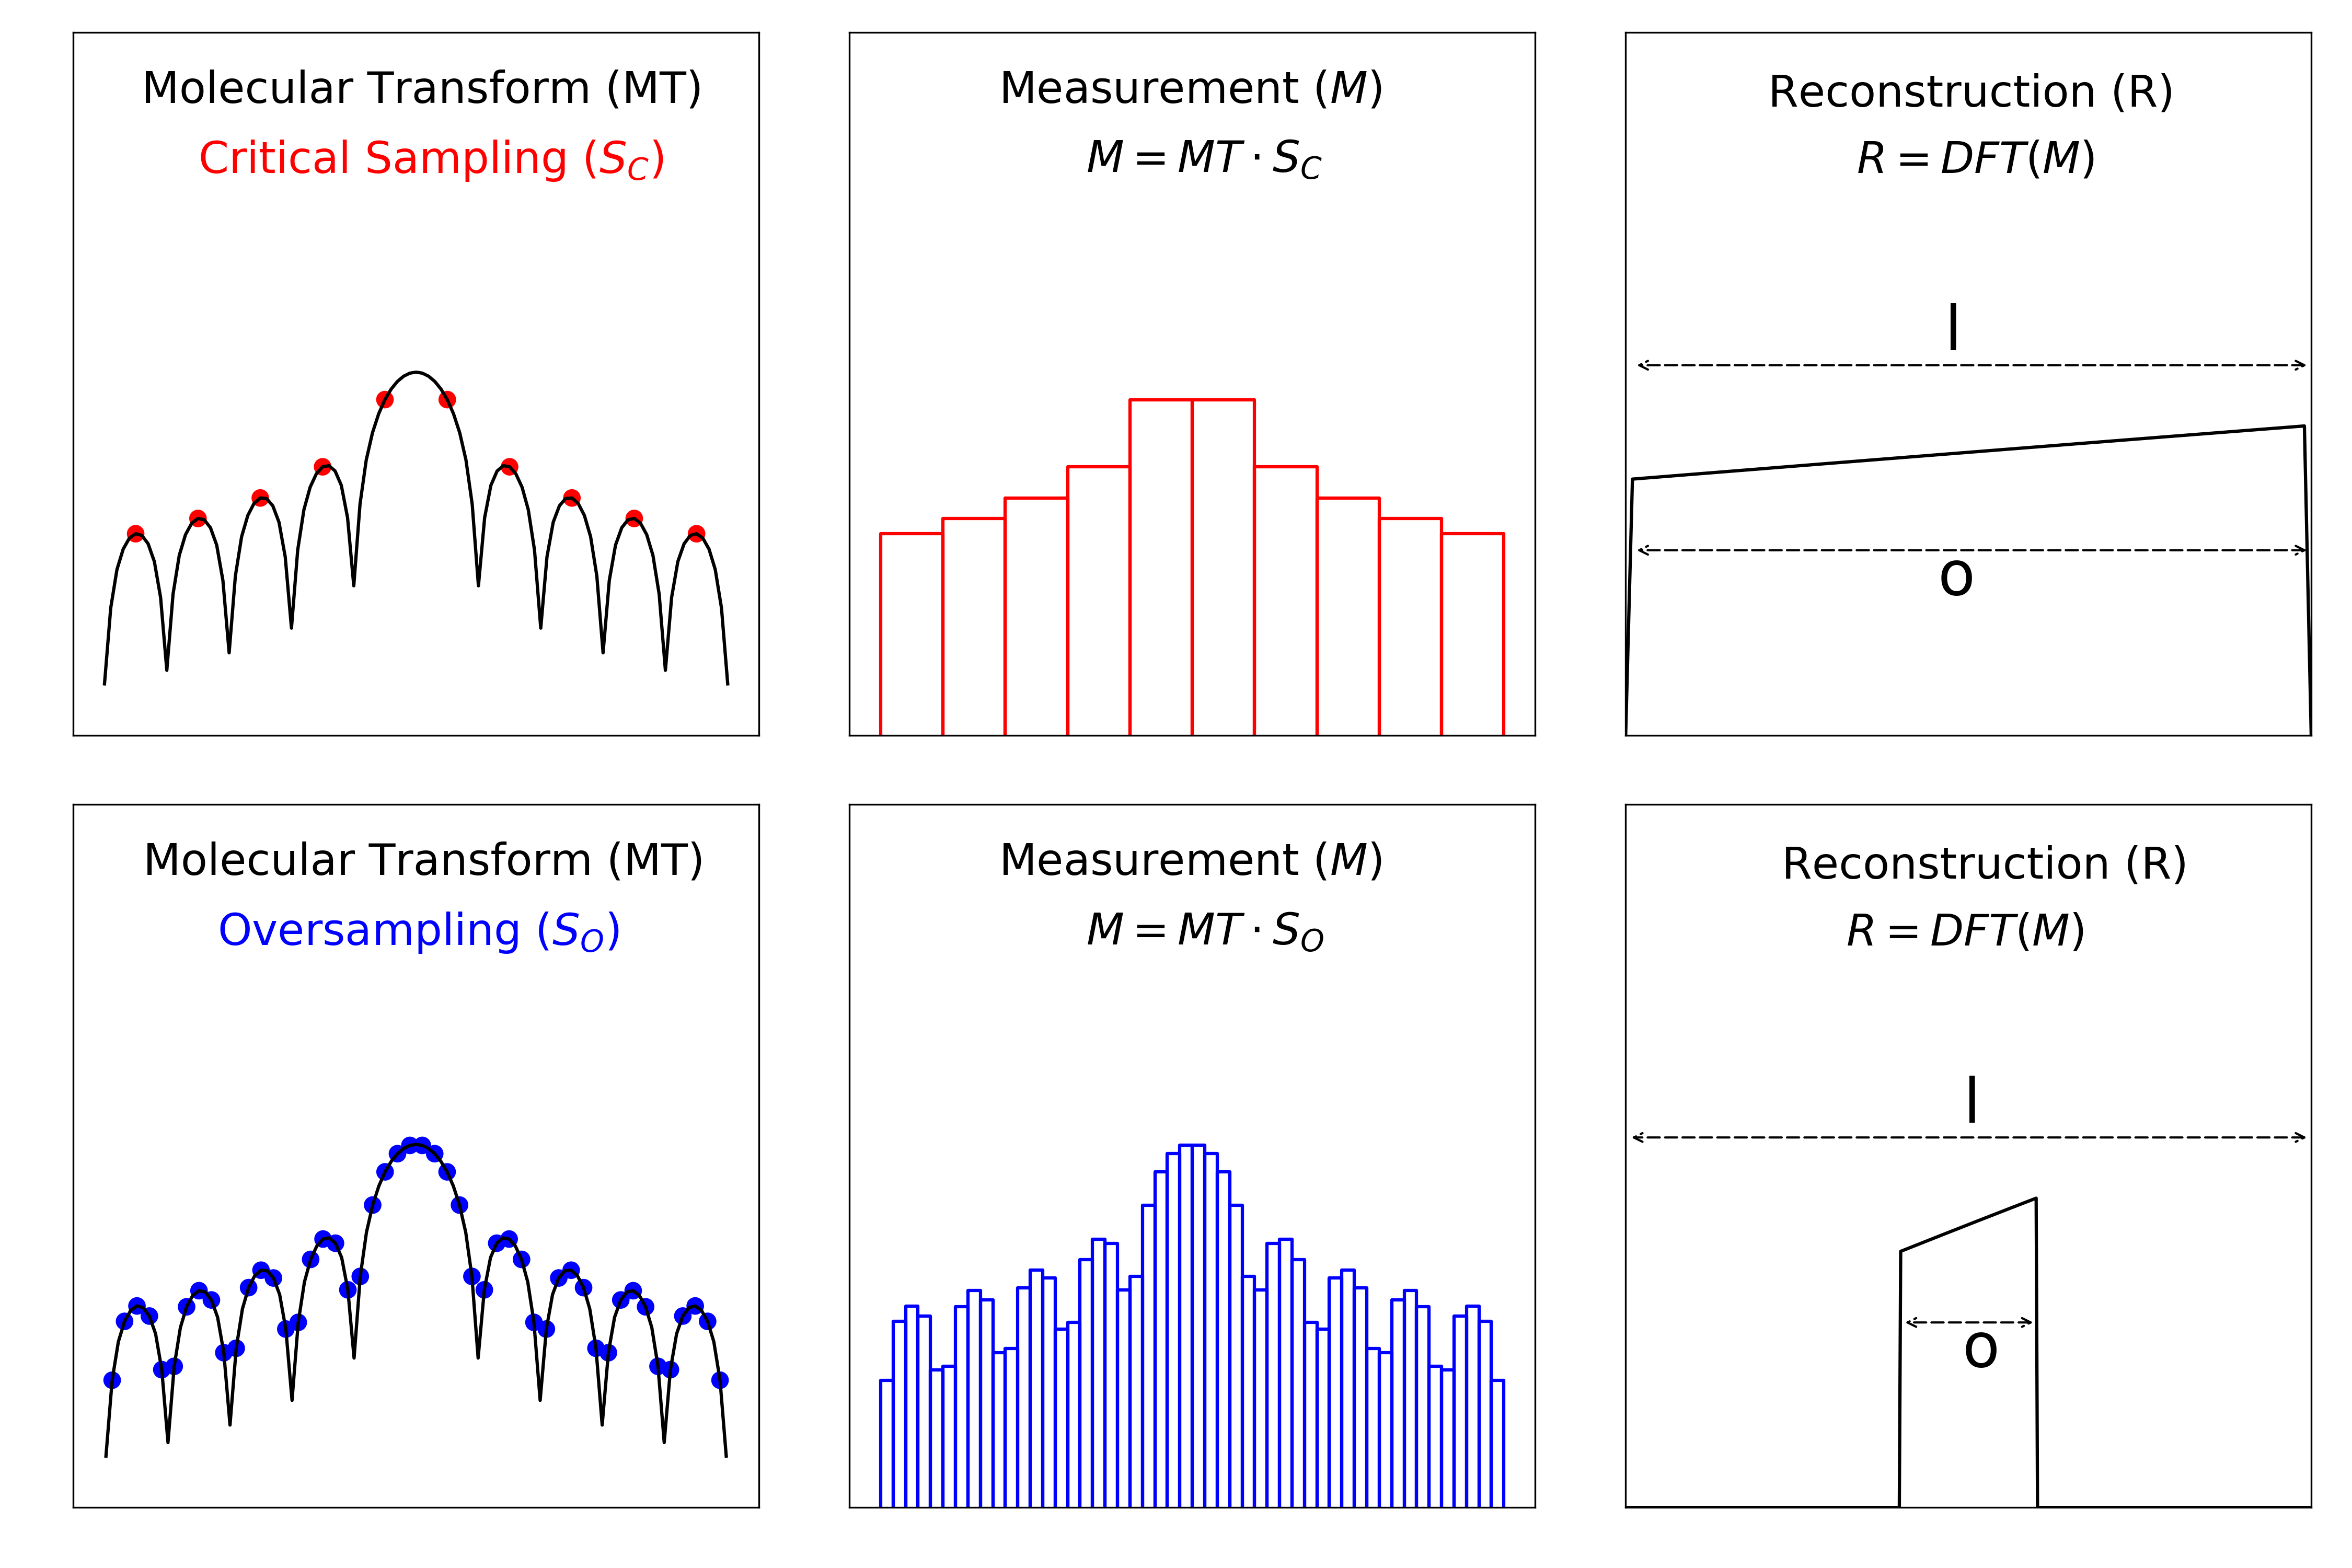
\includegraphics[width=120mm]{sampling.png}
	\caption{Illustration of critical sampling versus 		oversampling.}
	\label{fig:sampling}
\end{figure}

By choosing a detector setup such that the sampling rate is at least twice the critical sampling rate we can, in some cases, use the additional intensity information to recover the phases, and thus reconstruct the object from the measured intensities alone. It is known that this method does often does have multiple solutions in 1D \cite{Walther1963}, however, for higher dimensions it has been proven that, in most cases, an oversampled pattern will have a unique solution\cite{Bruck1979}. Oversampling is the basis of many phase retrieval techniques in SPI, as well as some clever phasing techniques in SFX \cite{Ayyer2016,Chapman2011}.

\section{Iterative Phase retrieval}
In practice there are many ways of actually retrieving the phase information from the diffraction pattern, but most common phase retrieval techniques are variations of convex optimization algorithms. This section introduces the general idea behind convex optimization, and explains the working three different algorithms. It has to be appreciated that solving the phases problem in remarkably difficult, as it is neither linear nor convex.

As with any difficult problem, one starts from the things that are known. Figure \ref{fig:sampling} shows that oversampling in Fourier space implies that there is an area the size of ($l-o$) around the object for which we know the electron density $\rho(\vec{r})$ is zero. This knowledge can be used as a constraint on the possible phases: we know that a correct choice of phases would make the corresponding $\rho(r)$ be zero in this area. The area that can contain positive electron density is called the support mask $M(\vec{r})$. This constraint is called the real-space constraint. Furthermore, we know that the recovered Fourier amplitudes should agree with the measured intensities. This is called the Fourier-space constraint. 

In 1978 Fienup \cite{Fienup1978}, inspired by an earlier algorithm by Gerchberg and Saxton [Gerchberg1972], introduced an algorithm called Error Reduction (ER) to solve the phase problem. ER is an iterative approach that tries to find the solution that minimizes the disagreement to both the real-space constraint and the Fourier constraint. In words it can be described as follows:\\
\begin{enumerate}
\item Assign random phases to each pixel.
\item Inverse Fourier transform F(s).
\item Set all electron density outside of $M$ to zero, keep other electron density.
\item Fourier transform $\rho(r)$
\item Make sure that the recovered amplitudes match the measured intensities. Keep the phases.
\item Go back to step 2.\\
\end{enumerate}


ER is sometimes able to find the correct solution, but because the problem is not convex, in general it often gets stuck in local minima, making ER unable to find the global solution.

In 1984 Levi and Stark realized that applying the above described constraints can be interpreted as projections in a multidimensional Hilbert space \cite{Stark1984}. Step 3 will from now on will be called the real-space projection $P_r$. A combination of step 4,5 and 2 will be called the Fourier Projection $P_f$.  In ER $P_r$ and $P_f$ can be defined as follows:
\begin{align}\label{eq:ER}
P_r \rho\left(\vec{r}\right) =& \begin{cases} \rho\left(\vec{r}\right) \quad &\mathrm{if}\,\,
    \vec{r} \in M\\0 \quad & \mathrm{if}\,\, \vec{r} \not\in M \end{cases}\\
P_f \rho(\vec{r}) =& \mathcal{F}^{-1}\left( \frac{\sqrt{I}}{|\mathcal{F}(\rho(\vec{r}))|}\mathcal{F}(\rho(\vec{r})) \right)
\end{align}

The largest difference between both projections is that the support constraint is convex, while the Fourier constraint is not. An iteration in ER can now been seen as a real-space projection followed by a Fourier projection. This can be summarized as:
\begin{equation}
\rho_{n+1}\left(\vec{r}\right) = \begin{cases} P_f\rho_{n}\left(\vec{r}\right) \quad &\mathrm{if}\,\,
    \vec{r} \in M\\0 \quad & \mathrm{if}\,\, \vec{r} \not\in M \end{cases}
\end{equation}

Two error metrics can be associated with both projection;the fourier error ($E_f$) and the real space error ($E_r$). $E_r$ is the fraction of density outside the support. $E_f$ shows the difference between the recovered amplitudes and the square root of the intensities. Mathematically $E_f$ and $E_r$ are defined as:

\begin{equation}
E_r = \left|P_r\rho(\vec{r}) - \rho(\vec{r})\right| = \left(\sum_i\rho_i^2\right)^{\frac{1}{2}}
\end{equation}

\begin{equation}
E_f = \left|P_f\rho(\vec{r}) - \rho(\vec{r})\right| = \left(\sum_{i}\left(\frac{\sqrt{I_i}}{|F(S_i)|}- F(S_i)\right)\right)^{\frac{1}{2}}
\end{equation}
  
\subsection{The Hybrid Input Output algorithm (HIO)}
In 1982 Fienup introduced an algorithm that can escape from local minima, the so-called the Hybrid Input Output algorithm (HIO). To achieve this HIO makes use of a so called relaxation parameter $\beta$. An iteration in HIO can be described as follows:
\begin{align}
\rho_{n+1}\left(\vec{r}\right) = \begin{cases} P_f \rho_{n}\left(\vec{r}\right) \quad &\mathrm{if}\,\,
    \vec{r} \in M\\\rho_n(\vec{r}) -\beta P_f \rho_n(\vec{r}) \quad & \mathrm{if}\,\, \vec{r} \not\in M \end{cases}
\end{align}

I see the $\beta$ parameter similar to temperature in simulated annealing. If $\beta$ is large even deep local minima can be escaped. Unfortunately this also means the global minima might be missed as well. If beta is small HIO will miss fewer minima, but will have greater difficulty escaping from them. As long as a minimum is not perfect ($E_r$ and $E_f$ are not both zero), HIO will, however, eventually be able to escape \cite{Martin2010}.

\subsection{The Relaxed Averaged Alternating Reflection algorithm (RAAR)}
Another algorithm that is used often in the work described in this thesis is the Relaxed Averaged Alternating Reflection algorithm (RAAR). RAAR does not escape all minima but it can escape shallower once. For high-quality data RAAR seems to find the solution quicker than HIO, and also in a more behaved manner. An iteration of RAAR can be described as follows:
\begin{align}
\rho_{n+1}\left(\vec{r}\right) = \begin{cases} P_f \rho_{n}\left(\vec{r}\right) \quad & \mathrm{if} \,\,
    \vec{r} \in M\,\mathrm{and}\,\rho_n(\vec{r}) \geq -(1+\beta)P_f\rho_n(\vec{r}) \\\
    \beta\,\rho_n(\vec{r}) -(1-2\beta) P_f \rho_n(\vec{r}) \quad & \mathrm{if}\,\, \mathrm{otherwise} \end{cases}
\end{align}

As both RAAR and HIO do not guarantee to end up in the bottom of a minimum, concluding phase recovery with a number of iteration of ER will ensure the bottom of the final minimum is found. This can improve the overall quality of the reconstruction, as shown in \textbf{Paper I}.

\subsection{Other algorithms}
There exist many other phase recovery algorithms. Examples are: diffusion map (DM) \cite{Elser}, GHIO[], HPR [], HAAR[] , ESPRESSO [], saddepoint optimisation [], and charge flipping []. A software package called Hawk allows users to select and test different algorithms. Hawk is especially powerful as it gives graphical feedback of the reconstruction process. This can for example be very useful to find the correct support size. 

\section{Validation}
In iterative phase retrieval every reconstruction results in an image, irrespective of it having biological relevance or not. It is therefore very important to have tools to validate a reconstruction. This section will describe different validation tools used in the field.

\subsection{Errors}
The most basic method to assess the difference in quality between two reconstructions is comparing the respective errors. The reconstruction with lower errors is generally considered to be a more successful reconstruction. This method however does not tell anything about the biological validity of a reconstruction and is most often only used to exclude outliers (reconstructions that have clearly failed).
 
\subsection{PRTF}
The standard tool to assess the quality of a reconstruction is the phase retrieval transfer function (PRTF). This function considers the variation within a set of independent reconstructions (each reconstruction starting from a random set of phases), and uses this variation to quantify the resolution of a reconstruction. The basic assumption behind the method is that if a similar object is retrieved repeatedly, this object is supposed to be similar to the true object. The variation between reconstructions is calculated for each pixel $i$ by adding all recovered amplitudes for that pixel and dividing the total vector by square root of the measured intensity for that pixel $v_i = |\frac{\sum A_i}{\sqrt{I_i}}|$. If the value of $v_i$ is close to unity all reconstructions recovered a similar amplitude for pixel i. The closer $v_i$ is to zero the more difference there is between individual reconstructions. The standard PRTF plot shows the radial average of $v_i$. A common practice is the field is to define the resolution of a reconstruction as the first time the 1D PRTF drops below $\frac{1}{e}$. This threshold is arbitrary. For spherical objects a periodic drop in the 1D PRTF, corresponding to a drop in measured intensity, can be observed. This drop can be explained by the fact that the phase of a pixel measuring 0 intensity is unconstrained.
 
\subsection{Missing Mode Analysis}
As described in previous sections diffraction patterns lack data. Even in the best case the central region will be missing because the direct beam will otherwise damage the detector. The main other sources of missing data are detector geometry and saturation. 

Reconstruction algorithms deal with this missing data by recovering the phase as well as the amplitude for the pixels in these regions. In many cases the missing data does not affect the stability of phase recovery, however this cannot be said in general. For this we have to note that the Fourier constraint does not limit the amplitudes in the missing data area, and the real-space constraint does not limit the electron density inside the support. If there exists an object that can fit inside the support and has a Fourier transform that is zero outside the missing data region, this object could be arbitrarily added to the solution and thus would form an ambiguity in the reconstruction process.

In general completely unconstrained objects do not exist. Objects that fit the support constraint and only slightly contribute outside the missing data region, i.e. weakly constrained objects, can however exist. In the design of an experiment, or when deciding whether or not to phase an object it is important to have a tool that predicts whether weakly constrained objects exist or not. Missing mode analysis is such a tool.

The DFT can be represented in matrix form, where each column represents a pixel in real space and each row represents a pixel in Fourier space. The rows and columns can be reordered according to whether they conform to the fourier and real space constraints or not.

\begin{equation}\label{equ:F_split}
  \mathcal{F} = 
  \left(\begin{array}{l|lll}
    \mathcal{F}_{SM} & &\mathcal{F}_{\bar{S}M}& \\\hline
    &&&\\
    \mathcal{F}_{S\bar{M}} & & \mathcal{F}_{\bar{S}\bar{M}} &\\
    &&&
  \end{array}\right)
\end{equation}

We are after objects that minimize $|\mathcal{F}_{SM}\rho|$. A common method to find such objects is singular value decomposition [Eckart]. This method decomposes $|\mathcal{F}_{SM}\rho|$ into a diagonal matrix $\Sigma$, and two unitary matrices U and V in the following way.

EXPLAIN EIGENVALUES AND BASIS




\subsection{Hierarchical clustering}
To test whether the Fourier Error and Real space error are good measures to assess the variance between individual reconstructions, a clustering analysis can be performed. An example of such an analysis is UPGMA (Unweighted Pair Group Method with Arithmetic Mean) hierarchical clustering [Sokal, Michener]. This method checks the similarity between reconstructions by making pairwise pixel-to-pixel comparisons between all reconstructions. The similarity score is the normalized scalar product between a pair reconstructions after translating them to their optimal fit. We plot the similarity score of  each cluster as a function of the number of clusters and choose the agglomeration step where the plot makes a "kink". This is a standard way to estimate the number of clusters present in the set of reconstructions. This capability is an advantage of the UPGMA clustering algorithm. In a 2D plot of FE vs RE, color-coded by cluster, it is possible to see whether or not there is a correlation of reconstruction similarity and error score. An illustration of this method can be found in \ref{fig:UPGMA}
 
\begin{figure}[h]
	\centering 
		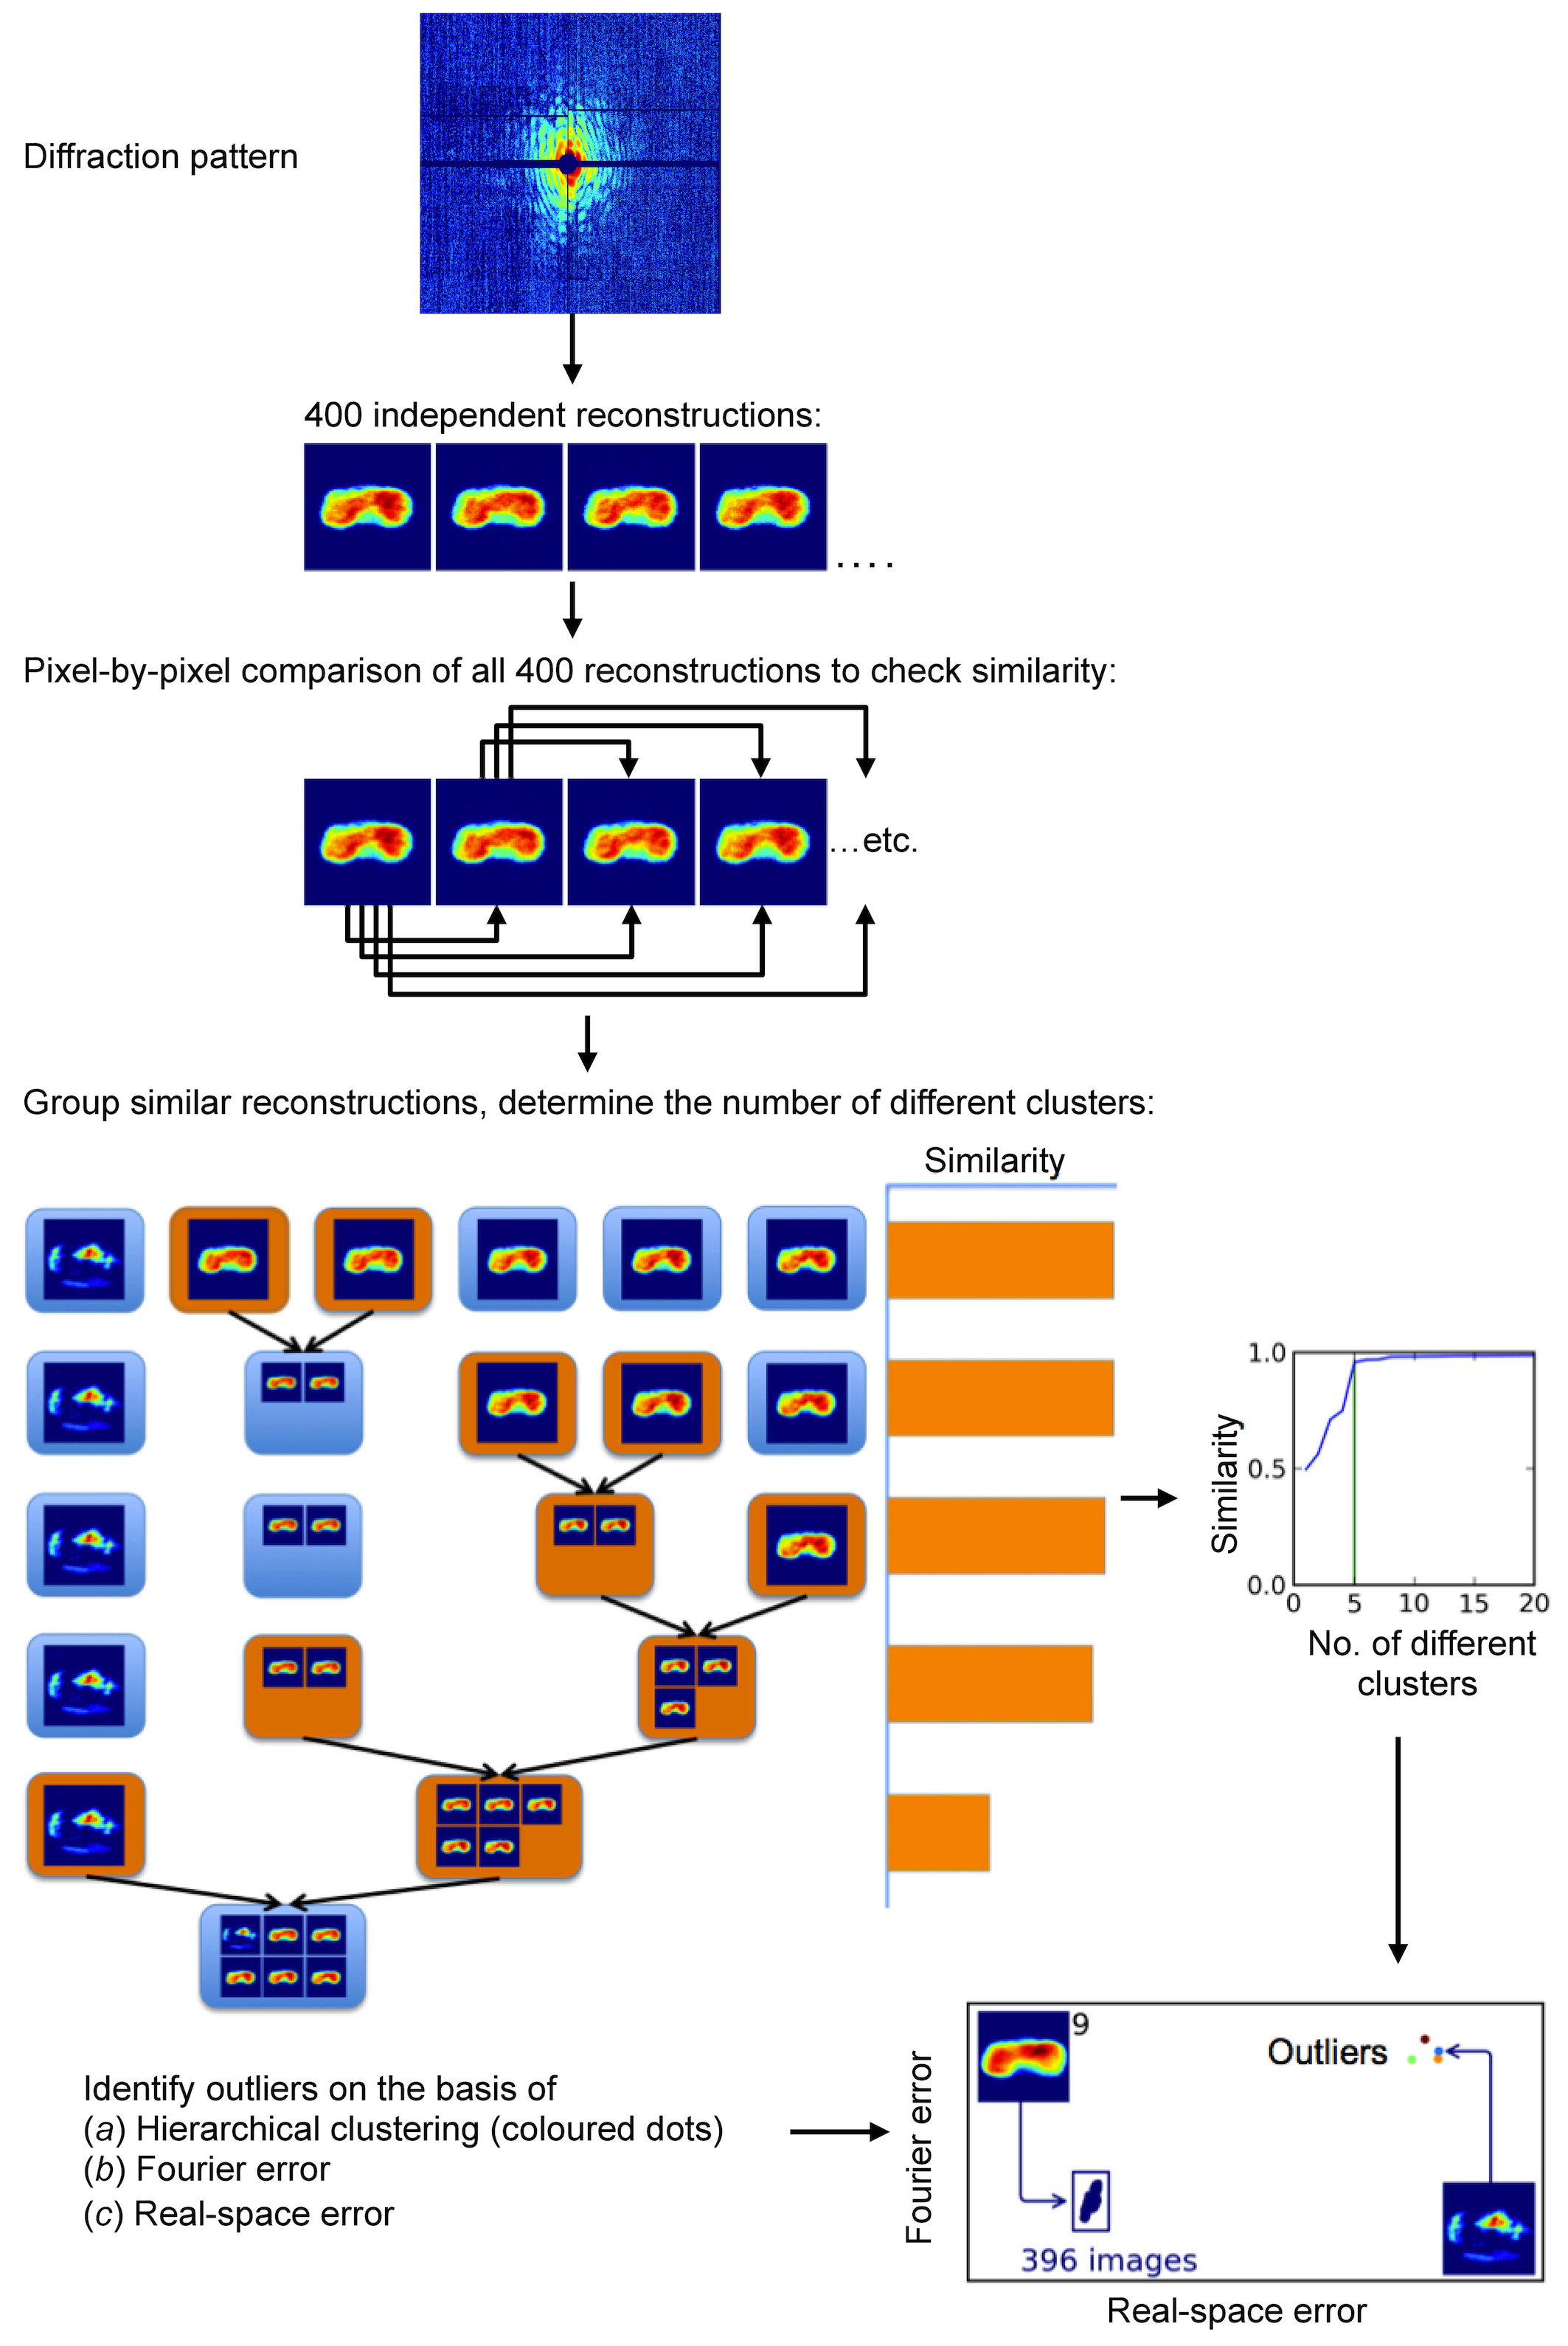
\includegraphics[width=100mm]{UPGMA_Clustering.jpg}
	\caption{UPGMA Clustering.}
	\label{fig:UPGMA}
\end{figure}

In the case that several large clusters remaining after applying a real-space error and Fourier-error threshold the clusters have to be examined carefully. If the remaining clusters correlate with the errors we suggest to keep only the cluster with the lowest error. If no correlation is present between score and cluster it is advised to keep all clusters for further evaluation. Otherwise there is a possibility of selecting on similarity, which would negate the validation power of the PRTF.

 
\section{Simulated Phase Contrast Methods}
Once one has retrieved the phase of the diffraction pattern, one has complete knowledge of the information encoded in the said wave-field. This total knowledge is powerful, because it allows the emulation of the action of any imaging system for which an associated mathematical transform can be written, regardless of whether that system is experimentally realizable in hardware.

For example, differential interference contrast imaging or Nomarski imaging is experimentally a well established technique to visualize the changes in phase. This change can have biological meaning, as for example the density inside certain organelles can be higher than the average density in cells. Normarski imaging will give a more pronounced image of the borders of the organelle. For an example see ref [mitochondrium). 

Nomarkski imaging in its simplest form takes a coherent wave-field of interest, say $\psi(x,y,z = 0)$, and then interferes this wave-field with a copy of itself that has been given both a slight transverse displacement ($\Delta x$, $\Delta y$) and a phase shift $\phi_0$ (Nomarski and Weill,1955). Thus the intensity of the resulting wave-field is [Paganin]:
$|\psi(x,y,z=0)+ e^{(i\phi_0)} \psi(x - \Delta x,y - \Delta y,z=0) |^2$, from which one can show (using the Fourier shift theorem) that the transfer function becomes:
\begin{equation}
\begin{aligned}
\begin{split}
T_{DIC}(k_x, k_y, \tau) = 1 + e^{(i(\phi_0 - k_x \Delta x - k_y \Delta y))},\\
\tau = (\phi_0, \Delta x, \Delta y)
\end{split}
\end{aligned}
\end{equation}

In the case of a reconstructed image $\rho(\vec{r})$, the Normarski variant will look like:
\begin{equation}
N = \mathcal{F}^{-1} T_{DIC} \mathcal{F}(\rho(\vec{r}))
\end{equation}
We have created simulated Nomarski images of the reconstructed cell images shown in the results part.

\section{Shrinkwrap}
While HIO and RAAR perform well when the support is tight and well known, phasing can practically become impossible if the support is too large. In 2003 Marchesini developed an algorithm that does not require a priori known support as input, but instead tries to deduce the shape of the support during the reconstruction. It starts by guessing the support from the autocorrelation. It does so by blurring the autocorrelation and selecting all pixels above a certain threshold to be included in the support. Consecutively after each n iterations the support is updated by applying a Gaussian blur to the real space image and selecting the pixels that have a value above a certain threshold. By varying the amount of blur and/or the selection threshold as the iterations progress, the support can slowly wrap and shrink to the true shape of the object. The general idea behind the algorithm is that even with a non-accurate support some features will be recovered well, and by using these features finally the an accurate support will be found. The algorithm has been very successful for experimental data [].

\chapter{3D restructions}
So far we have dealt with 2D diffraction patterns. Although much can be learned (and has been learned) from 2D images, having a structural 3D model is essential to understand the functioning of biomolecules. From the Fourier slice theorem we know that a diffraction pattern is a 2D slice through the center of the 3D diffraction pattern of the object. Different slices could therefore build up the 3D fourier transform of the object. In the current CXI setup it is impossible to image one object multiple times, making it difficult to reconstruct the complete 3D diffraction volume from one particle alone. If the particle of interest is reproducible the diffraction pattern from each copy could be used to construct the 3D fourier transform of the object. This does pose a new problem: the relative orientation of each diffraction pattern compared to the others has to be recovered. A variety of reconstruction algorithms have been proposed for recovering the relative orientation of diffraction data, including the EMC algorithm [Loh], the manifold embedding algorithms [Giannakis], simple best-fit models [Tegze], and multi-particle cross-correlation analysis [Saldin, Kirian, Kam, Kurta]. Theoretical studies suggest that the determination of diffraction pattern orientation should be possible even with very low photon counts of as little as 1000 scattered photons per image [Loh], making EMC and ME very suitable to recover the 3D structure of sparsely scattering single proteins.

\section{the EMC algorithm}
The EMC algorithm is an iterative program. On the one side you have the 2D measured intensity patterns ($IM_i$), and on the other side a 3D model of the Fourier space of the object ($M$). Each iteration starts with the expand step in which the 3D model is expanded in n central 2D slices ($IP_i$). N is dependent on the sampling rate of the 3D model. Each of the slices are compared to each diffraction pattern, using a model for the noise, to predict a probability score that the measured diffraction pattern is coming from the model diffraction pattern. To paraphrase: imagine that you would image each particle at the same orientation, the measured diffraction patterns will not be identical, since the noise is varying from shot to shot. Each pixel however will have an associated distribution of measured intensity values. Based on this distribution, which can for example be Poissonian in the case of pure shot noise, one can assign a probability that $IM_i$ is coming from slice $IP_i$. In  a good model not only will the measured values for a given 3D pixel (voxel) be similar for different $IM$, the distribution of measured values will have to be similar to the known noise distribution. This is a very subtle idea and utilizes the data very efficiently.

Comparing all $IM_i$ to each $IP_i$, lead to n probability distributions predicting the likelihood of the orientation of the measured diffraction patterns. This step is called the maximize step. Using the probability distributions as weights, a new model $M_{n+1}$ is generated from the measured diffraction patterns in the so-called compress step. 
The initial model $M_0$ can be a random model. After one iteration a similar patterns will end up in similar orientations which hopefully will make $M_1$ a bit more similar to the real Fourier pattern of the particle. After repeating this Expand-Maximize-Compress cycle multiple times a realistic model might be generated.

\section{Non-reproducible objects}
The addition of diffraction patterns from non reproducible object (i.e. incoherent addition) is very problematic in Fourier space space [Maia], as all features of the resolution of variation will be washed out. This makes it very difficult to retrieve 3D information from an heterogeneous object such as cells and the fold of many proteins. The tackle the heterogeneity problem many adaptations of existing algorithms or new algorithms have been developed.

\subsection{Multi-model EMC}
Currently a version of EMC is on its way that can generate multiple models of the same particle. It is very similar to single state EMC, but differs in the fact that it build multiple self-consistent models. 

\section{the Manifold Embedding algorithm}


\subsection{Tomography and sub-tomogram averaging}
Tomography used a set-up in which the object is imaged from m different but known orientations. Sometimes this is enough to gain enough information about the object in 3D. Crowther's criterion describes the relation between resolution and number of required exposures (m). For large objects and/or high resolutions it becomes difficult to have enough exposures to recover the full object at atomic resolution. In this case one could use multiple low resolution parts of the tomogram (sub-tomogram) to build up a model of semi-repoducible object in a method similar to EMC. The limit of the number of beams (m) for which this is possible in an XFEL setup is currently under investigation.

\subsection{Holography}
At high resolutions the detector does not measure the Ewald sphere and the Friedel symmetry of the diffraction pattern breaks. This is often very visible at longer wavelengths (<400 eV). This curvature can be exploited to resolve semi-3D information about the object, but the extend at which this is possible is disputed. In some cases much is known about the possible shape or buildup of the particle and then it is possible to reconstruct a 3D structure [Miao, Fennel, ...]

\chapter{Image Classification}
In order for algorithms such as EMC to work, the amount of heterogeneity within the diffraction data set has to be limited [TOMAS is there an article describing this?]. Furthermore, each of the steps in the experiment introduces it own type of noise to the measured diffraction pattern. For example think of the debris clumping around small particles compared to the drop when sprayed with the GDVN, detector malfunctioning or saturation, or intensity fluctuations due to the random start of the SASE process. Often the results of the first two types of noise can not be tolerated by EMC, and image classification before the EMC step is necessary. Also fast feedback about the first type of noise is very useful to have during the experiment. So far a very robust sizing method has been developed, but more extended methods might come in useful. Several methods shown here can give rapid feedback on the heterogeneity of the particle.

\section{Template-based classification}
If your object has a known shape it could be possible to only select the diffraction patterns that are similar to a set of expected diffraction patterns from the object called templates. Paper III explores the possibility of template-based classification. In general this method is highly dependent on the choice of template, as well as the amount and type of variation present in your sample.

\section{Feature extraction}
Another way of selecting diffraction patterns is by extracting general features from the diffraction pattern such as size, particle shape, amount of saturation, number of particles in the beam. Based on the relative values associated with the features patterns might be selected or not, or the experimental conditions might be rapidly adjusted. This section describes several methods to extract features.

\subsection{Size}
A common method to determine the size of an object is fitting the central speckle to the central speckle of simulated diffraction pattern from a sphere. This method has shown to be successful for particles that have an icosahedral shape to spherical shape \cite{Hantke2014,Daurer2017}. If the diffraction pattern also has the 3rd to the 5th minima present, the average of these minima can also be used to describe the size of the object. This method might be especially useful for strong scatterers, because the central speckle or first minimum might not be reliable due to saturation effects.

It might also be possible to determine the size and shape of an object from a filtered autocorrelation. This is useful when the object cannot be approximated by a sphere, but is rather elongated in one axis. Due to aerosol injection, the strongest contrast in the object is coming from the edge of the object. Therefore the edge is often one of the most clear features in an autocorrelation. This method is limited to convex objects.

\subsection{Multiple scatterers in the focus}


\subsection{Edge detection}
Some objects are characterized by having sharp edges. A sharp edge in real space corresponds to a streak in the direction perpendicular to the edge in Fourier space. Objects and/or orientations of objects might be classified by determining if streaks are present, and how many. Figure explains the idea behind a streak finding algorithm described in paper IV.


\chapter{Software}
\section{RedFlamingo}
